
%使用xelatex编译
%版权所有,翻版必究
%本文件由程序自动生成,任何修改将被覆盖
%2019 年 01 月 09 日




%

\FloatBarrier
\subsection{
在Windows平台下搭建开发环境
}\label{s000110}


\FloatBarrier
\subsubsection{
在Windows平台下安装Qt
}\label{ss000110}


读者可以到 \url{http://download.qt.io/archive/
}
下载最新的Qt运行环境。
然而,遗憾的是,从Qt 5.12.0开始从此网址下载的Windows平台下的Qt开发环境并不完整。
%介绍如何下载在线安装包...
读者不得不访问Qt官网 \url{https://www.qt.io
},
注册Qt帐号,然后按照流程下载在线安装包。
不得不说,这对初学者很不友好。
幸运的是,目前Qt网站有一个漏洞。读者可以直接访问
 \url{https://www.qt.io/download-thank-you
},点击“here”下载在线安装包。如\figurename\ \ref{p000000}。
%begin图片
\begin{figure}[htb] %浮动体 here and top ...
%there must use marginnote not use marginpar ...
\marginnote{\fbox{\footnotesize{\figurename\ \ref{p000000}}}}\centering %中心对齐
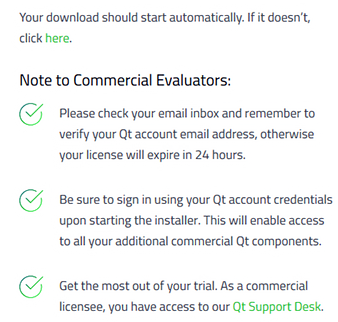
\includegraphics[scale=0.95]{chapter01/images/windows_download_here.png} %图片路径
\caption{Qt在线安装包下载路径} %标题
\label{p000000} %索引
\end{figure}
%end图片

以管理员身份运行在线安装包,
选择安装路径时请不要选择包含空格和中文字符的路径。
虽然现代开发环境对于空格和中文字符支持良好,
但是,很多第三方辅助工具未必支持空格和中文字符。
包括本书自带的辅助工具也不保证支持空格和中文。

在Windows平台下,建议读者选择安装“MSVC 2017 64\hspace{0.05em}\rule[0.7ex]{0.4em}{0.65pt}\hspace{0.05em}bit”或以上版
或者
“MinGW 7.3.0 64\hspace{0.05em}\rule[0.7ex]{0.4em}{0.65pt}\hspace{0.05em}bit”或以上版本。
Qt选择5.12.0或以上版本。
安装的时候最好选择安装“Sources”、“Qt Charts”、“Qt WebEngine”以及
“Qt Debug Information Files”这些模块。
在“Tools”选项下组好安装“CDB”以及对应的“MinGW”。
本书建议最小安装如\figurename\ \ref{p000001}。
%begin图片
\begin{figure}[htb] %浮动体 here and top ...
%there must use marginnote not use marginpar ...
\marginnote{\fbox{\footnotesize{\figurename\ \ref{p000001}}}}\centering %中心对齐
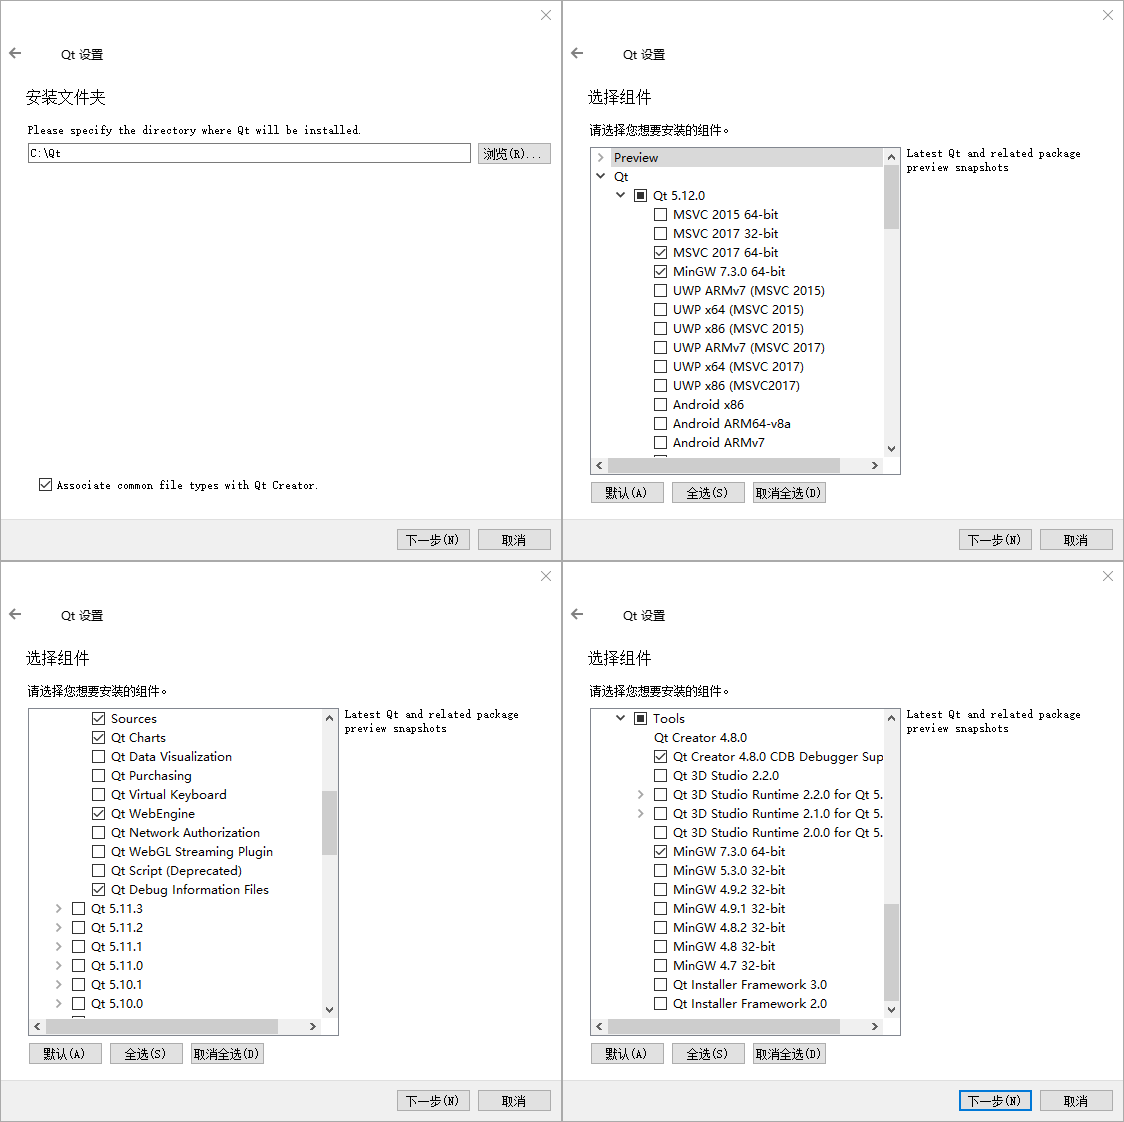
\includegraphics[width=0.95\textwidth]{chapter01/images/windows_qt_online_install.png} %图片路径
\caption{Qt在线安装建议选择安装组件} %标题
\label{p000001} %索引
\end{figure}
%end图片


\FloatBarrier
\subsubsection{
在Windows平台下安装Boost
}\label{ss000210}

读者只需要到Boost官网 \url{https://www.boost.org/
}下载最新Boost稳定版。解压缩,将“boost”文件夹复制到Qt Include路径即可。
比如,
用户的Qt Include路径为:
\begin{littlelongworld}
C:\textbackslash{}Qt\textbackslash{}Qt5.12.0\textbackslash{}5.12.0\textbackslash{}msvc2017\underline{\hspace{0.5em}}64\textbackslash{}include
\end{littlelongworld}
复制完boost之后,
应当存在路径:
\begin{littlelongworld}
C:\textbackslash{}Qt\textbackslash{}Qt5.12.0\textbackslash{}5.12.0\textbackslash{}msvc2017\underline{\hspace{0.5em}}64\textbackslash{}include\textbackslash{}boost
\end{littlelongworld}
\hspace*{\parindent}当然,读者也可以采用“mklink”建立链接代替拷贝。

\FloatBarrier
\subsubsection{
在Windows平台下MinGW配置jemalloc
}\label{ss000310}


%LD_PRELOAD
%由于Windows平台下不存在类似于Linux平台“LD_PRELOAD”这样可以动态
对于C{\sourcefonttwo{}+}{\sourcefonttwo{}+}来说,小对象的内存碎片问题向来很棘手。
一般而言,使用tcmalloc或jemalloc可以有效避免内存碎片问题。

在Linux平台或类似平台下,
可以使用“LD\underline{\hspace{0.5em}}PRELOAD”或类似的技术轻松的覆盖动态链接库中的函数。
因而,在Linux平台下,使用tcmalloc或jemalloc替换C库中的内存分配函数是简易的。

而在Windows平台下,
覆盖动态库中的函数相当复杂。
为了能够使得本书的示例代码不是玩具,
本书在Windows平台下使用jemalloc克服小对象内存碎片。

当使用MSVC编译器的时候,本书直接嵌入jemalloc源代码,
因而读者不必特别操心。
但是,当在Windows下使用MinGW编译器时,
读者需要自己静态编译jemalloc\footnote{
如果读者使用MinGW 7.3 64 bit版本的编译器,
本书已经将对应版本的jemalloc编译好了,
读者不需要再次编译。
}。
并将编译结果放置到:
\begin{littlelongworld}
QtQmlBook\textbackslash{}sstd\underline{\hspace{0.5em}}library\textbackslash{}memory\textbackslash{}libs
\end{littlelongworld}
文件夹下。
并将文件重命名为“jemalloc\underline{\hspace{0.5em}}win64\underline{\hspace{0.5em}}mingw\underline{\hspace{0.5em}}730.a”。
如果读者实在无法静态编译jemalloc,
读者可以找到:
\begin{littlelongworld}
QtQmlBook\textbackslash{}sstd\underline{\hspace{0.5em}}library\textbackslash{}\underline{\hspace{0.5em}}sstd\underline{\hspace{0.5em}}library\underline{\hspace{0.5em}}memory.pri
\end{littlelongworld}
并将此文件内容清空。


















%使用xelatex编译
%版权所有,翻版必究
%本文件由程序自动生成,任何修改将被覆盖
%2019 年 01 月 09 日



